\section{Getting started}
\label{gettingstarted}
This section gives an overview of Romeo, including the following paragraphs:
\begin{itemize}
\item \textbf{Installation and uninstallation}
\item \textbf{Main window}
\item \textbf{Environment}
\end{itemize}

\subsection{Installation}
\label{installation}
This paragraph will guide you through the installation procedure of Romeo.

\subsubsection{System requirements}
\label{systemrequirements}
To use the Romeo software, is necessary to have a computer running Windows 7; both 32 and 64 bit architecture are supported. Romeo also needs K-Lite codec pack, provided within the installer; if you already have this codecs, you could step their installation. There is no requirements on the amount of RAM nor on the CPU speed, but few hardware resources could compromise the efficiency of the application.

\subsubsection{Installation process}
\label{installationpriocess}
To install the product in your machine, follow these instructions:
\begin{itemize}
\item Execute the \textit{RomeoInno.exe} installer, by double clicking it;
\begin{figure}[!h]
\begin{center}
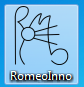
\includegraphics[scale=1]{./Images/icon}
\caption{\textit{Program installation icon}}
\label{visualizesubjectimg}
\end{center}
\end{figure}
\item Windows could ask you to confirm the installation, by showing the following dialog: \textit{"Do you want to allow the following program from an unknown publisher to make changes to this computer?"}. Confirm and continue;
\item The installation wizard starts. First of all, you must accepts the license agreement (Romeo is distributed under the \textbf{GNU General Public License v2.0}). Then select \textit{Next} fig.\ref{license};
\begin{figure}[!h]
\begin{center}
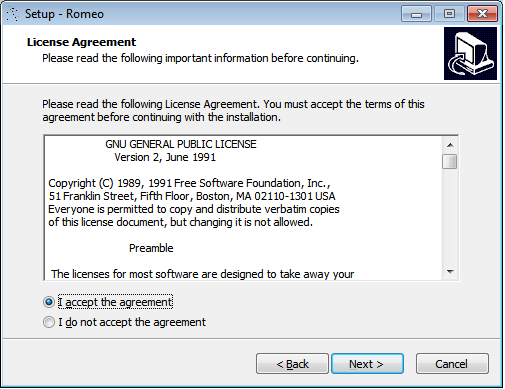
\includegraphics[scale=0.7]{./Images/licenza}
\caption{\textit{License agreement}}
\label{license}
\end{center}
\end{figure}
\pagebreak
\item Choose the folder in which you want to install Romeo. You can decide to not create a Start Menu folder by checking the flag, as in fig.\ref{folder}. Select \textit{Next};
\begin{figure}[!h]
\begin{center}
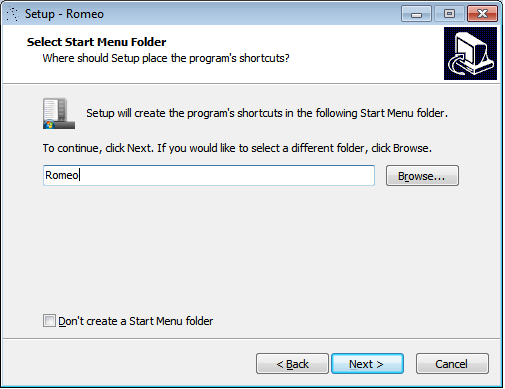
\includegraphics[scale=0.7]{./Images/folder}
\caption{\textit{Choosing the installation folder}}
\label{folder}
\end{center}
\end{figure}
\item Choose if you want to create a desktop icon, by clicking the relative flag, then select \textit{Next};
\item Select the \textit{Install} button. The installation will start (fig.\ref{install_romeo});
\begin{figure}[!h]
\begin{center}
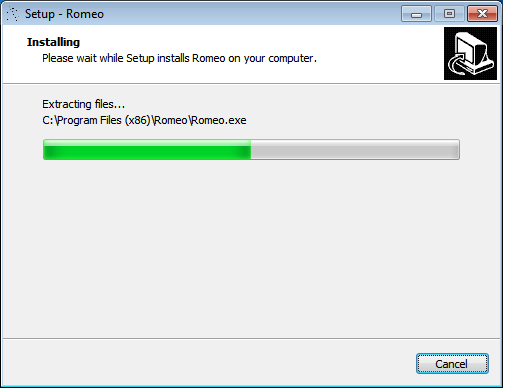
\includegraphics[scale=0.7]{./Images/installing}
\caption{\textit{Installation of Romeo}}
\label{install_romeo}
\end{center}
\end{figure}
\pagebreak
\item Once it will be completed, you must install the K-Lite codec pack, if they are not already present in the system. Uncheck the "Launch Romeo" flag and check the "Install Codec" one (fig.\ref{finish}). Step the following points otherwise;
\begin{figure}[!h]
\begin{center}
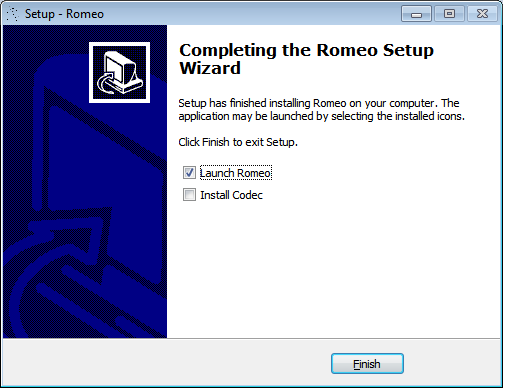
\includegraphics[scale=0.7]{./Images/finish}
\caption{\textit{End installation wizard}}
\label{finish}
\end{center}
\end{figure}
\item The installation wizard will appear; select the \textit{Next} button;
\item Select the \textit{Simple mode} installation option then confirm with \textit{Next} (fig.\ref{codecmode});
\begin{figure}[!h]
\begin{center}
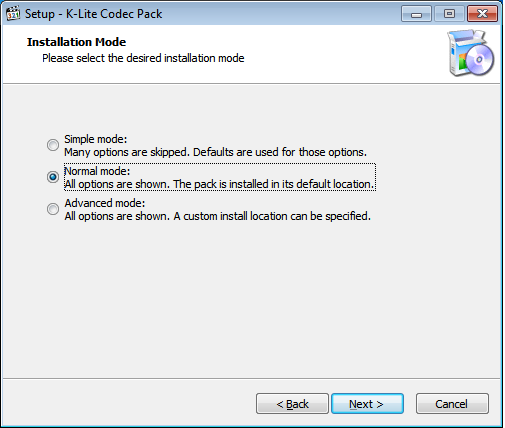
\includegraphics[scale=0.7]{./Images/codec_mode}
\caption{\textit{Choosing the codecs installation mode}}
\label{codecmode}
\end{center}
\end{figure}
\pagebreak
\item Continue following the wizard and then confirm the installation. Once it has finished, the \textit{Done} window will appear (fig.\ref{finish_codec});
\begin{figure}[!h]
\begin{center}
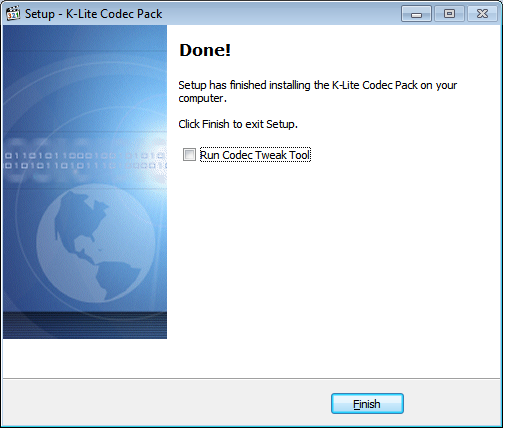
\includegraphics[scale=0.7]{./Images/codec_finish}
\caption{\textit{End codec installation wizard}}
\label{finish_codec}
\end{center}
\end{figure}
\end{itemize}

\subsection{Main window}
\label{mainwindow}
The Romeo main window includes two major panels. As you can see in fig. \ref{workareaimg}, the left panel contains a set of buttons, which will allow you to enter the windows that create and manage the entities of the software (Subjects\g{}, group of Subjects\g{}, Protocols\g{} and Datasets\g{}). The right panel, contains the \textbf{Analysis} section wich includes two buttons that will bring you respectively to the analysis execution window and the results visualization window.\\
The \textbf{More Help} section, instead, includes the links to access the informative materials of the software:
\begin{itemize}
\item 
\includegraphics[scale=0.06]{./Images/manual} Opens the User Manual of Romeo;
\item 
\includegraphics[scale=0.06]{./Images/videoguide} Brings to the video tutorial of Romeo;
\item 
\includegraphics[scale=0.06]{./Images/shortcuts} Shows the keyboard shortcuts;
\item 
\includegraphics[scale=0.085]{./Images/about} Shows informations about Romeo and its developers.
\end{itemize}
\begin{figure}[!h]
\begin{center}
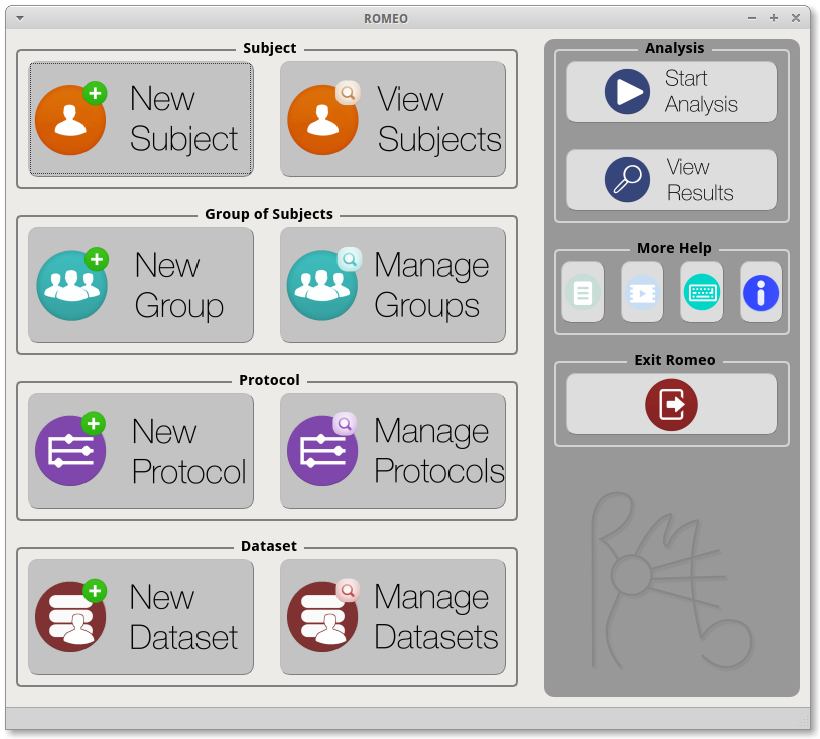
\includegraphics[scale=0.4]{./Images/MainWindow}
\caption{\textit{Main window of Romeo}}
\label{workareaimg}
\end{center}
\end{figure}

\subsection{Environment}
\label{environment}
The windows of Romeo, except the Main Window, have a Menu Toolbar on their top, which includes the direct links to all of the functionalities of Romeo.
\begin{figure}[!h]
\begin{center}

\includegraphics[scale=0.5]{./Images/MenuToolbar}
\caption{\textit{Menu Toolbar}}
\label{menutoolbar}
\end{center}
\end{figure}
You can drag and drop this Toolbar on the left or right of the window. Below, the explanation of the various buttons (see fig \ref{menutoolbar}):
\begin{itemize}
\item 
\includegraphics[scale=0.085]{./Images/home} Brings back to the main window;
\item 
\includegraphics[scale=0.08]{./Images/new_Subject} Leads to the \subject{} creation window (see \ref{createsubject});
\item 
\includegraphics[scale=0.08]{./Images/manage_Subjects} Leads to the \subject{} visualization window (see \ref{visulizesubjects});
\item 
\includegraphics[scale=0.08]{./Images/new_Group} Leads to the group of Subjects\g{} creation window (see \ref{creategroup});
\item 
\includegraphics[scale=0.08]{./Images/manage_Groups} Leads to the groups of Subjects\g{} managing window (see \ref{managegroups});
\item 
\includegraphics[scale=0.08]{./Images/new_Protocol} Leads to the \protocol{} creation window (see \ref{createprotocol});
\item 
\includegraphics[scale=0.08]{./Images/manage_Protocols} Leads to the Protocols\g{} managing window (see \ref{manageprotocol});
\item 
\includegraphics[scale=0.08]{./Images/new_Dataset} Leads to the \dataset{} creation window (see \ref{createdataset});
\item 
\includegraphics[scale=0.08]{./Images/manage_Datasets} Leads to the Datasets\g{} managing window (see \ref{managedataset});
\item 
\includegraphics[scale=0.07]{./Images/start_Analysis} Leads to the Analysis window (see ref{analysiswindow});
\item 
\includegraphics[scale=0.07]{./Images/show_Results} Leads to the Results window (see ref{resultswindow}).
\item 
\includegraphics[scale=0.085]{./Images/exit} Exit from Romeo;
\end{itemize}
Furthermore, this button is present in every window: 
\includegraphics[scale=0.08]{./Images/help} It will provide informations about the functionalities of the current page.